


\tikzset{every picture/.style={line width=0.75pt}} %set default line width to 0.75pt        

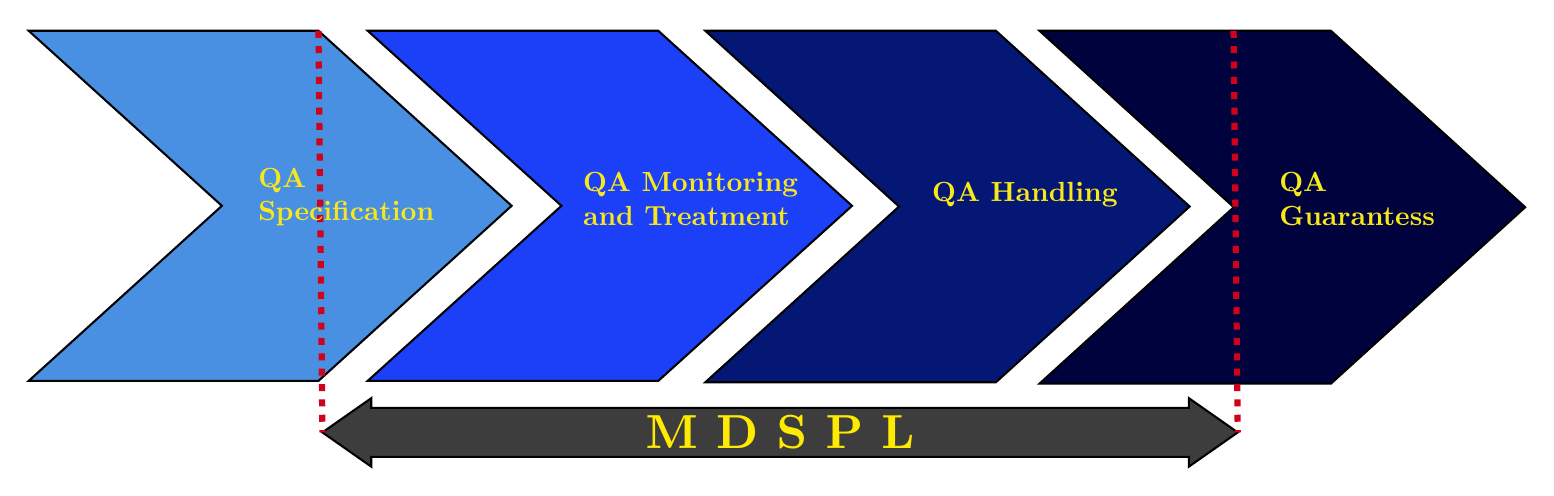
\begin{tikzpicture}[x=0.75pt,y=0.75pt,yscale=-1,xscale=1]
%uncomment if require: \path (0,268); %set diagram left start at 0, and has height of 268

%Chevron Arrow [id:dp7998116230156174] 
\draw  [fill={rgb, 255:red, 28; green, 64; blue, 248 }  ,fill opacity=1 ] (180.33,40) -- (320.33,40) -- (413.67,124.33) -- (320.33,208.67) -- (180.33,208.67) -- (273.67,124.33) -- cycle ;
%Chevron Arrow [id:dp17326121534239214] 
\draw  [fill={rgb, 255:red, 74; green, 144; blue, 226 }  ,fill opacity=1 ] (17,40) -- (156.6,40) -- (249.67,124.33) -- (156.6,208.67) -- (17,208.67) -- (110.07,124.33) -- cycle ;
%Chevron Arrow [id:dp2103753298875829] 
\draw  [fill={rgb, 255:red, 5; green, 23; blue, 117 }  ,fill opacity=1 ] (343,40) -- (483,40) -- (576.33,124.67) -- (483,209.33) -- (343,209.33) -- (436.33,124.67) -- cycle ;
%Chevron Arrow [id:dp7759460284870137] 
\draw  [fill={rgb, 255:red, 0; green, 2; blue, 61 }  ,fill opacity=1 ] (504,40) -- (644.4,40) -- (738,125) -- (644.4,210) -- (504,210) -- (597.6,125) -- cycle ;
%Left Right Arrow [id:dp5098219629430656] 
\draw  [fill={rgb, 255:red, 7; green, 7; blue, 7 }  ,fill opacity=0.78 ] (158.5,233.5) -- (182.05,217) -- (182.05,221.71) -- (575.95,221.71) -- (575.95,217) -- (599.5,233.5) -- (575.95,250) -- (575.95,245.29) -- (182.05,245.29) -- (182.05,250) -- cycle ;
%Straight Lines [id:da7722048533467026] 
\draw [color={rgb, 255:red, 208; green, 2; blue, 27 }  ,draw opacity=1 ][line width=2.25]  [dash pattern={on 2.53pt off 3.02pt}]  (156.6,40) -- (158.5,233.5) ;


%Straight Lines [id:da37299757229242914] 
\draw [color={rgb, 255:red, 208; green, 2; blue, 27 }  ,draw opacity=1 ][line width=2.25]  [dash pattern={on 2.53pt off 3.02pt}]  (597.5,40) -- (599.5,233.5) ;



% Text Node
\draw (170,120) node [color={rgb, 255:red, 248; green, 231; blue, 28 }  ,opacity=1 ] [align=left] {\textbf{QA}\\\textbf{Specification}};
% Text Node
\draw (336,121) node [color={rgb, 255:red, 248; green, 231; blue, 28 }  ,opacity=1 ] [align=left] {\textbf{QA Monitoring}\\\textbf{and Treatment}};
% Text Node
\draw (657,121) node  [align=left] {\textbf{\textcolor[rgb]{0.97,0.91,0.11}{QA }}\\\textbf{\textcolor[rgb]{0.97,0.91,0.11}{Guarantess}}};
% Text Node
\draw (497,119) node  [align=left] {\textbf{\textcolor[rgb]{0.97,0.91,0.11}{QA Handling}}};
% Text Node
\draw (379,233.5) node [scale=1.7280000000000002,color={rgb, 255:red, 255; green, 235; blue, 0 }  ,opacity=1 ] [align=left] {\textbf{M D S P L}};


\end{tikzpicture}